\documentclass[a4paper,10pt]{article}
\usepackage[utf8]{inputenc}
\usepackage{tikz}
\usetikzlibrary{chains,intersections}
\renewcommand*{\familydefault}{\sfdefault}
\begin{document}

%styles
\tikzset{thegrid/.style = {help lines, color = #1!50,very thin, step = 0.5cm}, thegrid/.default = blue}

%draw a square (executes everyting until semicolon)
\tikz \draw[thick,rounded corners=0pt]
(0,0) -- (0,2) -- (2,2) -- (2,0) -- (0,0);

%draw some coordinate axes (uses different environment, draws everything within env.)
\begin{tikzpicture}
 \draw (-1.5,0) -- (1.5,0);
 \draw (0,-1.5) -- (0,1.5);
 \draw (-1,0) ..controls (-0.5,1) and (0.5,1) .. (1,0);
\end{tikzpicture}

%basic figure
\begin{tikzpicture} [scale = 3]
 \draw [thegrid = red] (-1.4, -1.4) grid (1.4, 1.4);
 \draw [<->] (-1.5,0) -- (1.5,0);
 \draw [<->](0,-1.5) -- (0,1.5);
 \draw (0,0) circle (1cm);
 \filldraw[fill=green!20!white, draw=green!50!black]
(0,0) -- (3mm,0mm) arc (0:30:3mm) -- cycle;
\draw[red, very thick] (30:1cm) -- +(0,-0.5);
\draw[blue, very thick] (30:1cm)  ++(0,-0.5) -- (0,0);

\foreach \x/\X in {-1, -0.5/-\frac{1}{2}, 0.5/\frac{1}{2}, 1}
  \draw (\x cm, 1pt) -- (\x cm, -1pt) node[anchor = north, fill = white] {$\X$};
\foreach \y/\Y in {-1, -0.5/-\frac{1}{2}, 0.5/\frac{1}{2}, 1}
  \draw (1pt, \y cm) -- (-1pt, \y cm) node[anchor=east, fill = white] {$\Y$};
\end{tikzpicture}

%clip of basic figure (use \clip[draw] to simultaneously clip and draw)
\begin{tikzpicture} [scale = 6]
\clip (-0.1, -0.2) rectangle (1.1, 0.75);
 \draw [thegrid = red] (-1.4, -1.4) grid (1.4, 1.4);
 \draw [<->](-1.5,0) -- (1.5,0);
 \draw [<->](0,-1.5) -- (0,1.5);
 \draw (0,0) circle (1cm);
 \shadedraw[left color=gray,right color=green, draw=green!50!black]
(0,0) -- (3mm,0mm) arc (0:30:3mm) -- cycle;
\draw[red, very thick] (30:1cm) -- +(0,-0.5);
\draw[blue, very thick] (30:1cm)  ++(0,-0.5) -- (0,0);

\foreach \x/\X in {-1, -0.5/-\frac{1}{2}, 0.5/\frac{1}{2}, 1}
  \draw (\x cm, 1pt) -- (\x cm, -1pt) node[anchor = north, fill = white] {$\X$};
\foreach \y/\Y in {-1, -0.5/-\frac{1}{2}, 0.5/\frac{1}{2}, 1}
  \draw (1pt, \y cm) -- (-1pt, \y cm) node[anchor=east, fill = white] {$\Y$};
\end{tikzpicture}



% A curved path

\tikz \draw (0,0) .. controls (1,1) and (2,1) .. (2,0)
	    (0,0) .. controls (1,-1) and (2,-1) .. (2,0);

% some circles
\tikz \filldraw [fill = orange, draw = black] (0,0) circle (10pt);

% nodes

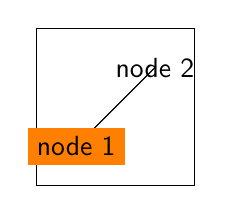
\begin{tikzpicture}
 \draw (0,0) rectangle (2,2);
 \draw (0.5, 0.5) node [fill=orange]
 {node 1} -- (1.5, 1.5) node {node 2};
\end{tikzpicture}


\end{document}